% Sample file for 'CACM - Research Highlights'-type articles
% Created by: Gerry Murray, Elec. Pub. Info. Mgr., Pubs. Dept., ACM HQ, NY.
% (murray@hq.acm.org)
%
% This is "research-highlights-sample.tex" (sample file) V1.1 Sept. 2008
% This file should be compiled with V1.1 of "research4cacm.cls" Sept. 2008
%
% If you have already submitted an article to an ACM/SIGS Conference, and have had your
% article published in one of the 'Proceedings', then you have probably used
% the (ACM/SIGS) 'sig-alternate' class and .tex file.
% Any such 'conference-prepared' source .tex file is 'compatible' with the class file
% 'research4cacm' which you will use to prepare your article for inclusion in the magazine 'CACM'.
%
% Here are the steps to take in order to 'morph' your article from being
% a 'conference' article to one more suitable for inclusion in 'Communications of the ACM'.
%
% 1. Change \documentclass{sig-alternate}  to \documentclass{research4cacm}
%
% 2. Comment out the conference information e.g.  %\conferenceinfo{WOODSTOCK}{'97 El Paso, Texas USA}
%
% 3. Make sure the copyright data is correct e.g. \crdata{0001-0782/08/0200}
%
% 4. Make sure the YEAR is correct e.g. \CopyrightYear{2008} with the current default being �2008�.
%
% 5. Comment out the Classification scheme, general terms and keywords.
%
% 6. If you have mentioned authors in the 'Additional Authors' section you should
%    'move them back' into the byline (so that they appear with all the other authors).
%    ALL authors, in Research Highlights articles, get equal billing.
%
% 7. Suitably edit the file (i.e. body text) so as to make it more appropriate for a wider audience.
%
% If, early on in the editorial process, the 'correct' copyright data becomes available
% please change the copyright data to suit, otherwise leave the default '0001-0782/08/0X00'.
% (The editorial staff will change it later on in the production cycle.)
%
% ================= IF YOU HAVE QUESTIONS =======================
% Technical questions _only_ to
% Gerald Murray (murray@hq.acm.org)
% ===============================================================
% ---------------------------------------------------------------------------------------------------------------
%
\documentclass{research4cacm}
\usepackage{graphicx}
\usepackage{listings}
\usepackage{enumitem}
\usepackage{hyperref}

\begin{document}


%
% --- Author Metadata here ---
% Conference information is NOT appropriate for CACM so comment it out.
%\CopyrightYear{2008} % Allows default copyright year (2008) to be over-ridden - IF NEED BE.
%\crdata{0001-0782/08/0X00}  % Allows default copyright data (0001-0782/08/0X00) to be over-ridden - IF NEED BE.
% --- End of Author Metadata ---

\title{The BBC micro:bit - from the UK to the World
% \titlenote{(This is a simple titlenote.)For use with research4cacm.cls. Supported by ACM.}
%
% Show use of \thanks - which can appear here (normal/default) or down by the author
%\thanks{thank someone?}
}
\subtitle{[Extended Abstract]
%\titlenote{A full version of this paper is available in...}
}
%
% You need the command \numberofauthors to handle the 'placement
% and alignment' of the authors beneath the title.
%
% For aesthetic reasons, we recommend 'three authors at a time'
% i.e. three 'name/affiliation blocks' be placed beneath the title.
%
% NOTE: You are NOT restricted in how many 'rows' of
% "name/affiliations" may appear. We just ask that you restrict
% the number of 'columns' to three.
%
% Use the \alignauthor commands to handle the names
% and affiliations.
%
\numberofauthors{3} %  in this sample file, there are a *total*
% of SIX authors and all of them fit neatly on the first page.
% As said, all authors get 'equal billing' and you should fit all of them on the opening page
% in the 'byline'. The production/editorial-staff will 'separate' names from their affiliations, leaving
% author names beneath the title (in the byline), and moving the affilations/contact information to an area
% after the references at the back of the article.
%
\author{
% You can go ahead and credit any number of authors here,
% e.g. one 'row of three' or two rows (consisting of one row of three
% and a second row of one, two or three).
%
% The command \alignauthor (no curly braces needed) should
% precede each author name, affiliation/snail-mail address and
% e-mail address. Additionally, tag each line of
% affiliation/address with \affaddr, and tag the
% e-mail address with \email.
%
% 1st. author
\alignauthor Lancaster University \\
\alignauthor Micro:bit Educational Foundation \\
\alignauthor Microsoft Research \\
    %    \affaddr{Institute for Clarity in Documentation}\\
    %    \affaddr{1932 Wallamaloo Lane}\\
    %    \affaddr{Wallamaloo, New Zealand}\\
    %    \email{trovato@corporation.com}
% 2nd. author
% 3rd. author
}

\maketitle
\begin{abstract}

The micro:bit rocks!

\end{abstract}

% The classification Scheme, General Terms and Keywords are not appropriate for CACM so comment them out.

\section{Introduction}
\label{sec:intrp}

In the early 1980's, the British Broadcasting Corporation (BBC)
introduced a whole generation of educators and students in the United Kingdon (UK)
to computing through the {\em BBC Computer Literacy Project}, which featured the BBC Micro,
a 6502-based personal computer designed and produced by Acorn Computers Ltd. (referred
to at times as the ``British Apple'').  The project was very sucessful:
more than 80\% of UK classrooms had a BBC Micro and many of today's
computing professionals from the UK first encountered computing through
the BBC Micro[REF].

Fast forward to 2015: the BBC sought to again inspire a new
generation get creative with coding, programming and digital technology
through its {\em Make It Digital} initiative, as well as to support the UK's mandate to
teach computer science concepts at all grade levels.~\cite{PeytonJones2013ICFP}

As part of this effort, the BBC introduced the micro:bit (see
Figure~\ref{fig:microbit}),
a small programmable and embeddable computer designed,
developed and deployed by the BBC and partners (including ARM, Microsoft
and Lancaster University) to approximately 800,000 UK middle school students
in 2015-2016. Harkening back to its work with the BBC Micro,
the BBC described the micro:bit as its ``most ambitious education initiative in 30 years,
with an ambition to inspire digital creativity and
develop a new generation of tech pioneers.''~\cite{BBCwebsite}

By embracing a simplified constructionist~\cite{Papert} approach to computing education, the micro:bit has moved from
a local educational experiment in the UK to a global phenomenon, now present in over 37 countries.
Driving the worldwide expansion is
the Micro:bit Educational Foundation (\url{www.microbit.org}),
a non-profit organization
established in September 2016, with the support of its founding partners~\footnote{ARM,
Amazon, BBC, British Council, IET, Lancaster University, Microsoft,
Nominet, and Samsung.}.
The Foundation's Mission Statement is to:
\begin{itemize}
\item  enable and inspire all children to participate in the digital world,
with particular focus on girls and those from disadvantaged groups.
\item make micro:bit the easiest and most effective learning tool for digital skills and creativity.
\item work in collaboration with educators to create and curate exceptional
curriculum materials, training programmes and resources.
\item build and support communities of educators and partners
to remove the barriers to learning digital skills
\end{itemize}

In this paper, we describe the key decisions and lessons from
delivering the BBC micro:bit in the UK and then expanding to reach
more educators and students around the world.
We draw from two full years of
full deployment of the micro:bit in the UK, as well as deployments
in Europe, the Americas, and Asia.  There are approximately
two million micro:bits now in the market and many hardware,
content, and education partners participating.

%Purpose
%- what is the micro:bit?
% http://www.bbc.co.uk/programmes/articles/4hVG2Br1W1LKCmw8nSm9WnQ/the-bbc-micro-bit


% reference the competition and show what's different (hardware)
% https://barrettsprojects.wordpress.com/2012/09/15/tap-and-double-tap/

\begin{figure}
  \begin{tabular}{cc}
    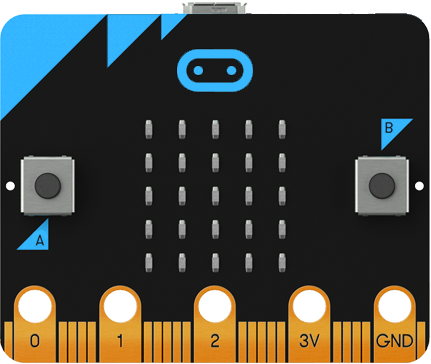
\includegraphics[width=1.5in]{images/microbit-front.png} &
    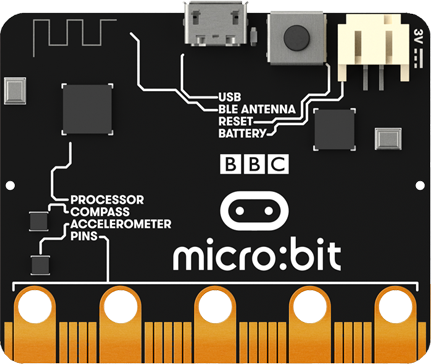
\includegraphics[width=1.5in]{images/microbit-back.png} \\
    (a) & (b)
  \end{tabular}
  \caption{\label{fig:microbit}The micro:bit: (a) front, with two buttons,
    5x5 LED display, and edge connector (bottom); (b) back, with processor, accelerometer, compass, Bluetooth, USB and battery ports.}
  \end{figure}

  \begin{figure*}[t]
    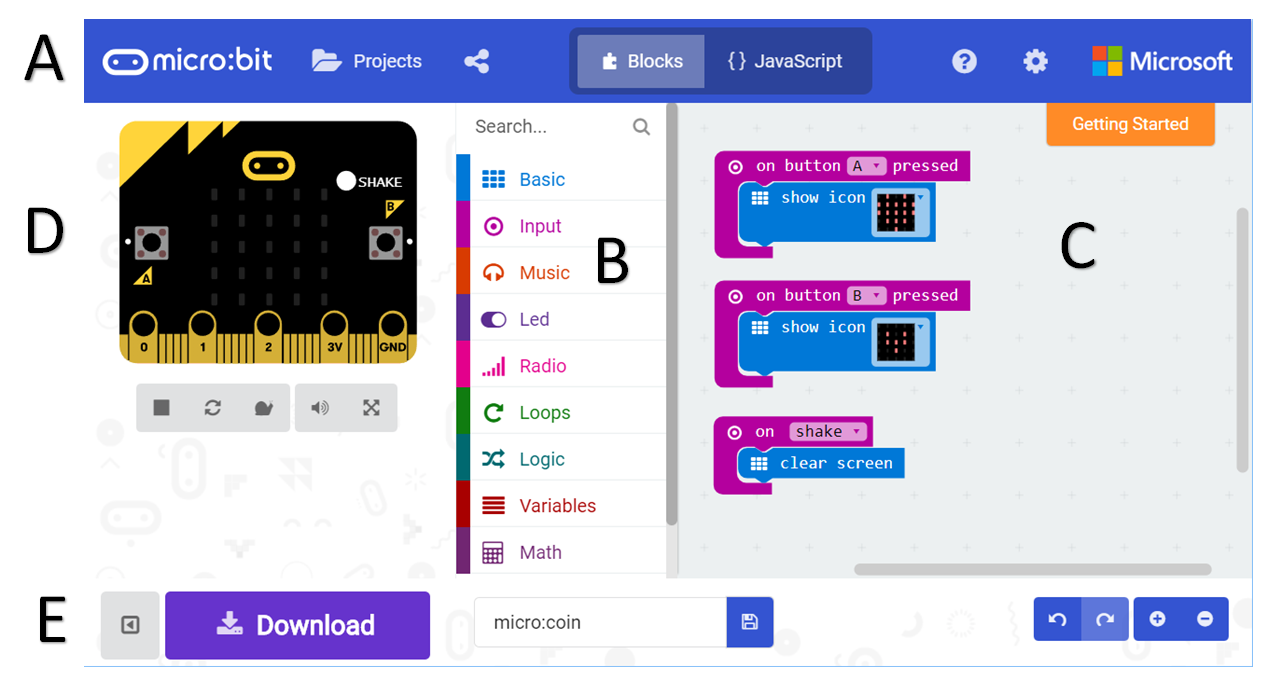
\includegraphics[width=6in]{images/webApp.png}
    \caption{\label{fig:snapshot}MakeCode web app for the micro:bit (\url{http://makecode.microbit.org}).}
  \end{figure*}

\subsection{Hardware}

Figure~\ref{fig:microbit} shows (a) the front and (b) the back of the
micro:bit, which measures 4cm x 5cm. Like the Arduino Uno~\cite{Arduino},
the micro:bit is a single-board microcontroller
that can be programmed via a host computer (usually a laptop or desktop)
and then embedded in projects where it runs on battery power.
In contrast to the Uno, which has no built-in sensors, the micro:bit
board hosts a variety of sensors (temperature, accelerometer, magnetometer,
light level),
a 5x5 LED matrix, two user-defined buttons, as well as Bluetooth
Low Energy (BLE) communications.\footnote{The micro:bit has a whopping
16kB of RAM and 256kB of Flash memory, compared to the Uno's 2kB of
RAM and 32kB of Flash}.

The design of the micro:bit hardware was driven by the
first two objectives of the BBC micro:bit project:
(B1) to provide a simple creative experience for physical computing, wearable and Internet of Things (IoT) projects;
(B2) to supply a device that can continue to provide learning opportunities as the user's expertise grows.

On the hardware side, the micro:bit's built-in sensors, buttons and LED display
allow many projects to be completed with no additional hardware or wiring.
The holes on micro:bit's edge
connector allows additional external sensors and actuators to be connected via crocodile clips.
The micro:bit's BLE capabilities introduces networking to the
picture, and enables streaming of data and command/control operations among the micro:bit,
smartphones, laptops, as well as other micro:bits.
As with Arduino, an ecosytem of micro:bit shields
(hardware peripherals) that accommodate the micro:bit's edge
connector expands its capabilities greatly (\url{http://microbit.org/resellers/}).

\subsection{Software}

The design of the micro:bit coding tools also was oriented towards a
simple starting experience with room for progression. In particular, the coding
objectives of the project were: (B3)
to give students an exciting, engaging introduction to coding;
(B4) to stimulate curiosity about how computing technologies can be utilized
  to solve problems that students identify.

Based on in-school trials with a micro:bit prototype, the BBC focused on delivering a web app
based on the popular Blockly framework~\cite{Blocky2015} to permit students to
create scripts via drag-and-drop operations in a web browser, and see
the execution of their scripts via a simulator.
Text-based coding via scripting languages also
was identified as an important feature. As the micro:bit would be incorporated
into standalone projects, it also was essential for the user's program to be
compiled and installed in non-volatile storage on the micro:bit where it
could be run via battery power.

%final design put the entire toolchain in web app, without need to invoke C/C++ compiler to
%compile the user's program; ARM DAPlink solution makes micro:bit appear as USB pen drive
%on all operating systems; MicroPython provided second programming solution with entire toolchain
%on the micro:bit!!]

% less techy here

The solution delivered by the BBC's partners evolved from the initial
design to include support for Blockly, JavaScript and Python, all
via web apps.
Figure~\ref{fig:snapshot} shows a screen snapshot of the MakeCode web app
for the micro:bit,
which supports programming via both Blocky and JavaScript.
The web app has five main sections: (A) menu bar with access to projects
and examples, and switching between Blockly and JavaScript editors; (B)
Blockly toolbox of micro:bit API categories; (C) Blockly programming
canvas with a simple reactive program; (D) micro:bit simulator for execution
of the user's program in browser; (E) download button, which invokes the in-browser
compiler/linker to produce a binary executable.

% The event-based program shown in section (C) displays a large heart when the
% A button is pressed, displays a small heart when button B is pressed,
% and clears the display when the user shakes the micro:bit (shake
% detection is implemented using the accelerometer; in the simulator, the
% shake event is fired using a virtual button). In addition to event-based
% APIs, direct access to the micro:bit's sensors via polling is possible.

The Python solution for the micro:bit is based on MicroPython (\url{http://micropython.org})
an implementation of Python 3.0 for microcontrollers. It includes
a full Python compiler and runtime that runs on the micro:bit and
supports a read-eval-print loop (REPL) to execute commands sent via
a terminal, as well as to import and run scripts from the Python web app for
the micro:bit (\url{http://python.microbit.org}).

% \begin{itemize}
% \item
% \item an efficient C++ runtime for the micro:bit created by Lancaster
% University;
% \item a web app
% with Blockly and JavaScript editors, micro:bit simulator,
% and a compiler to machine code (linked against a pre-compiled
% C++ runtime image, so no C++ compiler is needed for user code);
% \item a Python compiler and read-eval-print loop (REPL) that resides
% {\em on the micro:bit} (via \url{https://micropython.org/}),
% supported by a simple web app (\url{http://python.microbit.org}) and
% an installable application (\url{https://codewith.mu/});
% \item ARM's DAPlink firmware makes the micro:bit appear as USB pen drive
% on most operating systems, enabling a simple file copy operation to
% install a user's program on the micro:bit (no device drivers needed).
% \end{itemize}
% MakeCode, MicroPython, and the C++ runtime are all open source.\footnote{
% At \url{https://github.com/microsoft/pxt},
% \url{https://github.com/micropython/micropython},
% and \url{https://github.com/lancaster-university/microbit-dal},
% respectively.}


% \subsection{Content and training}

% The BBC micro:bit project also called for partners to develop content
% and to ``train the trainers'' (educators) around the micro:bit computing
% system.  This built on efforts by the non-profit Computing At Schools
% (\url{www.cas.org}) organization to train UK educators to teach computer
% science.

%- A lot of lessons learned from delivering end-to-end experience in UK and other countries
%   - hardware (unique design, as already mentioned)
%   - firmware:  high-level C/C++ runtime and ARM's DAPlink
%   - web-based IDE: no C/C++ compiler needed to compile user code
%   - content
%   - training
% In country partnerships

% main points
% - mass participation
% - country readiness (or perhaps willingness)

\subsection{Overview}

Section~\ref{sec:physical} reviews physical computing, which anchors
and defines the micro:bit experience. Section~\ref{sec:projects}
presents a broad set of micro:bit-based projects, ranging
from wearable games to environment science, that demonstrate
the micro:bit's capabilities.  Section~\ref{sec:country}
describes the rollout of the micro:bit in the UK and other countries
in Europe, the Americas and Asia. Section~\ref{sec:conclude}
concludes with final thoughts about what has made the micro:bit
successful to date and what comes next.


% compared to Arduino
% https://twitter.com/adamwwolf/status/1019070808038072320

% success of micro:bit due to
% - Low-cost, simplicity
% - Partnerships (hardware, software, content, training)
% - Open Source of software (CODAL, MakeCode, ...)
% - Hardware Reference design

% - why is it interesting?
%   - edge/physical/IoT computing
%   - build off of Scratch/Blockly, but untethered (via in-browser compiler)
%   - transition to JavaScript and Python

% - BBC rollout in UK
% - Global reach
%    - BBC rollout mirrored in other countries
%    - Communities
%      - Sri Lanka user group: http://microbitslug.org/
%      - UK libraries (loan program)
%    - third party editors










\section{Physical Computing}
\label{sec:physical}

As discussed in the Introduction, the micro:bit is a device
with similarities to the Arduino family of printed 
circuit boards. Such {\em physical computing} devices
are designed to be placed in and interact with our physical environment. 
Physical computing lives in the spaces between computing and many other disciplines:
art, industrial design, health, environmental monitoring; it has
close ties to cyber-physical systems, embedded systems, and IoT. The National
Science Foundation
defines cyber-physical systems as those that ``integrate sensing, computation, 
control and networking into physical objects and infrastructure, 
connecting them to the Internet and to each other.''\cite{NSF}


% from 
% "Cyber-physical systems "
%
% https://en.wikipedia.org/wiki/Embedded_system

{\bf TODO: this derived from Steve/Sue white paper - need to check carefully}.
The benefits of using physical computing to introduce beginners to computing systems include:
\begin{itemize}
\item {\em broad reach} because of diverse applications of physical computing -- leverage fine arts, music, design, etc. in projects;
\item {\em increased motivation} because of tangible visible outcome (rather than virtual on screen);
\item {\em learning by doing} as there are many ways to achieve goal (no single correct solution)
\item {\em natural division of labor} for more complex projects (design, hardware, software, ...)
\item {\em full system view of computing}: hardware and software working together.
\end{itemize}

\subsection{Wiring and Arduino}

% from thesis of Hernando Barragán:
% - http://people.interactionivrea.org/h.barragan/thesis/thesis_low_res.pdf 
% - Wiring: Prototyping Physical Interaction Design
% - June 2004

% http://wiring.org.co/

% https://globenewswire.com/news-release/2017/05/19/988294/0/en/Arduino-Welcomes-Hernando-Barrag%C3%A1n-as-Arduino-Chief-Design-Architect.html

To help explain the BBC micro:bit, it's very instructive to understand
Hernando Barragan's 2003 Master's thesis, ``Wiring: Prototyping Physical Interaction Design'',
the inspiration for the Arduino system~\cite{Barragan}. His objective was to make it easier
for non-technical creators, such as artists and designers, to leverage
electronics in their their work by simplifying the hardware and programming
experience. In particular, he said of existing work:
``Current prototyping tools for electronics and programming are mostly targeted 
to engineering, robotics and technical audiences.''  
Of Wiring's design, he identified the following key concepts:
\begin{itemize}
\item a simple cross-platform integrated development environment (IDE) to create so-called ``sketches'';
\item simplified application programming interfaces (APIs) to access a microcontroller's resources;
\item leverage open source compiler/linker toolchain, transparent to the end user;
\item a bootloader to make it easy to upload a compiled sketch to the microcontroller;
\end{itemize}
Also key to Wiring  was openness of both the hardware and software
comprising the system.

But, still some issues:
\begin{itemize}
    \item reliance on the C language and C compiler (needs to be installed)
    \item very poor experience in IDE
    \item USB bootloader requires device drivers on some systems 
\end{itemize}

% Uno: (which measures 5.34cm x 6.86cm),

\begin{figure} 
    \begin{tabular}{cc}
      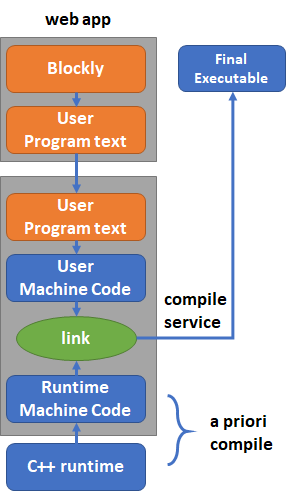
\includegraphics[width=1.5in]{images/bbc.png} & 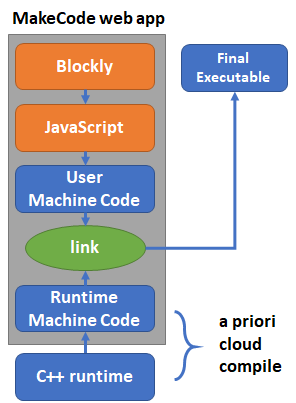
\includegraphics[width=1.5in]{images/makecode.png} \\
        (a) & (b) 
    \end{tabular}
    \caption{\label{fig:design}Web and compiler designs: (a) initial BBC design; (b) final design, as implemented in MakeCode.}
    \end{figure}

    
\subsection{The BBC micro:bit}

Main points:
\begin{itemize}
\item {\em A Visible Computer}: BBC micro:bit inherits the raw PCB nature of Arduino  (everything is visible to the end user).
\item {\em No Wiring}: makes starting easy
\item {\em Small Size}: 
\item {\em Scripting via Web App}: XYZ
\item {\em No Install}: XYZ
As shown in Figure~\ref{fig:design}(a), in the BBC design
the text of a user's program (whether derived from Blockly or produced directly by the user)
is submitted to a compile service that returns a final executable to be copied onto a micro:bit (connected to the host 
computer by USB) via a specialized loader application.  
avoiding the need for a compile service for user code (as shown 
in Figure~\ref{fig:design}(b));
\item {\em Extensible}: via edge connector and layered APIS (package system too). Note
that edge connector is a (male) plug - micro:bit plugs into to peripherals, not the
other way around.
\end{itemize}
From this perspective, the micro:bit can be seen as a starter device
for physical computing, embedded systems and cyber-physical systems, as it has
sensing, computation, control and networking capabilities built in.  The
micro:bit is not properly an IoT device, having no built-in way to connect
over IP, but it can be connected to other devices with IP connectivity. 

% Design considerations (technical requirements, steal from LCTES paper)

%   - hardware clearly distinguished from Arduino
%     - no wiring required to do interesting things (integrated sensors and outputs, etc.)
%     - device appears as USB pen drive (drag-and-drop programming)
 
%   - As with Arduino, embedding device into projects is essential (from beginner to maker)
%     - battery power
%     - works disconnected from host
%     - wearable, transportable
%     - low cost
%     - edge connector for easy connection to "shields"

%   - support for scripting languages (JavaScript and Python; no C/C++ for beginners)
%     - event-based programming model

%   - web-based IDE
%     - no apps or device drivers to install
%     - school considerations (minimize IT admin involvement)

%   - layered approach
%     - simple for absolute beginners to get started
%     - room for students to advance to more complex projects

% - worldwide rollout
%   - microbit.org, makecode.microbit.org

% from http://cacm.acm.org/system/assets/0000/6052/CACM_Author-Guidelines.pdf 

% 2.3.4 Contributed Articles
% Contributed Articles cover the wide and abundant spectrum of the computing field—its open challenges, 
% technical visions and perspectives, educational aspects, societal impact, significant applications and 
% research results of high significance and broad interest. 

% we have:
% + technical vision
% + educational aspect and societal impact
% + signification application
% - research results of high significance and broad interest: see LCTES 2018 article


% rollout
% - Canada: http://microbit.org/en/2018-03-13-cancode-microbit-funding/ 
% - Denmark: http://microbit.org/en/2018-05-07-dr-announcement/ 

%ACKNOWLEDGMENTS are optional
\section{Acknowledgments}

% The following two commands are all you need in the
% initial runs of your .tex file to
% produce the bibliography for the citations in your paper.
\bibliographystyle{abbrv} % standard abbrv style
\bibliography{paper}  % substitute the name of 'your' Bibliography here
% You must have a proper ".bib" file
% and remember to run:
% latex bibtex latex latex (in that particular order) in order to resolve all the 'numerical values'
% be they for figures, equation numbers, references, footnotes, etc. etc.
%
\balancecolumns
% That's all folks! % GM Sept. 2008
\end{document}
